% В этом шаблоне используется класс spbau-diploma. Его можно найти и, если требуется, 
% поправить в файле spbau-diploma.cls
\documentclass{spbau-diploma}
\begin{document}
% Год, город, название университета и факультета предопределены,
% но можно и поменять.
% Если англоязычная титульная страница не нужна, то ее можно просто удалить.
\filltitle{ru}{
    chair              = {Кафедра математических и информационных технологий},
    title              = {Анализ смесей близкородственных
бактериальных штаммов в метагеномных~сериях},
    % Здесь указывается тип работы. Возможные значения:
    %   coursework - Курсовая работа
    %   diploma - Диплом специалиста
    %   master - Диплом магистра
    %   bachelor - Диплом бакалавра
    type               = {master},
    position           = {студента},
    group              = 605,
    author             = {Аксешина Маргарита Дмитриевна},
    supervisorPosition = {к.\,ф.-м.\,н.???},
    supervisor         = {Нурк С.\,Ю.},
    reviewerPosition   = {ст. преп.},
    reviewer           = {Кто-то?? А.\,И.},
    chairHeadPosition  = {д.\,ф.-м.\,н., профессор},
    chairHead          = {Омельченко А.\,В.},
    % university = {САНКТ-ПЕТЕРБУРГСКИЙ АКАДЕМИЧЕСКИЙ УНИВЕРСИТЕТ},
    % faculty = {Центр высшего образования},
    % city = {Санкт-Петербург},
    % year             = {2013}
}
\filltitle{en}{
    chair              = {Department of Mathematics and Information Technology},
    title              = {Analyzing mixtures of closely related strains in metagenomic series data},
    author             = {Margarita Akseshina},
    supervisorPosition = {professor???},
    supervisor         = {Sergey Nurk},
    reviewerPosition   = {assistant},
    reviewer           = {Who??},
    chairHeadPosition  = {professor},
    chairHead          = {Alexander Omelchenko},
}


\maketitle


\tableofcontents


% ВВЕДЕНИЕ
\section*{Введение}

Метагеномика, -- раздел геномики, изучающий ДНК, извлеченную и отсеквенированную непосредственно из среды без этапа изоляции и культивирования отдельного вида. Метагеномика позволяет исследовать то, как отдельные микроорганизмы сосуществуют вместе, помогает понять функции и свойства сообществ. Например, средствами метагеномики можно отслеживать, как меняется и от чего зависит такая важная часть здоровья человека, как его микробиом \cite{HMP1, HMP2}. Кроме того метагеномика, -- это часто единственный шанс изучить организмы, которые слишком сложно, долго, дорого или попросту невозможно изолировать от их среды.

Одной из самых распространенных и легко доступных технологий для получения метагеномных данных является чтение ДНК с помощью секвенирования нового поколения, результатом которого является набор коротких геномных фрагментов, \--- ридов. Часто при этом в одном исследовании секвенируют сразу несколько связанных друг с другом образцов, собранных в разный момент времени \cite{time_series} или в разных местах \cite{spacial_series_1, spacial_series_2}.

Так как важные функциональные элементы генома (гены, регуляторные участки, повторы и т.д.) обычно не умещаются в один рид, чтобы проводить дальнейший анализ, эти короткие последовательности с помощью метагеномных сборщиков \cite{IDBA-UD, MEGAHIT, MetaVelvet, RayMeta, MetaSpades} объединяют в более длинные, \--- контиги. 

Чтобы оценить структуру популяции или восстановить геномы отдельных видов, используют методы биннинга, \--- то есть разделение метагеномных последовательности на группы так, чтобы в одной группе были последовательности только одного вида или, в крайнем случае, нескольких близкородственных. Как правило программы для биннинга \cite{CONCOCT, GroopM, MyCC, MetaBAT} кластеризуют последовательности, основываясь на их геномном составе (например, тетрануклеотидном спектре) и их покрытии в каждом из образцов. В тех алгоритмах, где используется сходство между профилями покрытия последовательностей в образцах, длина серии играет существенную роль в улучшении качества результатов биннинга.

Для выяснения таксономического состава образцов можно использовать инструменты, которые выравнивают последовательности на известные референсные геномы целиком \cite{GOTTCHA, CLARK, Kraken} или только на маркерные гены \cite{MetaPhlAn2, mOTU}. К сожалению, такой подход не позволяет выявить те организмы, которые не присутствуют в базах.

Вышеперечисленные подходы работают в основном на уровне видов. Если в данных присутствуют близкородственные штаммы, сборка получается сильно фрагментированной, или контиги будут соответствовать только доминантному организму. Из-за схожести геномного состава программы биннинга будут группировать близкородственные штаммы вместе. 

Но многие исследования (такие, например, как секвенирование изолятов) показывают, что важные свойства микроорганизмов могут различаться внутри одного вида. Анализ штаммо-специфичных особенностей генома позволяет выяснять функциональные и патогенные свойства микроорганизмов (например, среди Escherichia coli встречаются как штаммы-симбионты человеческого кишечника, так и патогенные \cite{patogen_ecoli} и карциногенные \cite{carcinogenic_ecoli}, проводить ассоциации генов с фенотипом хозяина (например, различные штаммы  Helicobacter pylori ассоциируются с различным риском развития  рака желудка \cite{cancer_example}, отслеживать краткосрочные эволюционные события (например, появление резистентности к антибиотику \cite{antibitics_resistance}).

Существует несколько методов, в которых риды выравниваются на референсные гены или геномы, чтобы выяснить вариации на уровне штаммов de novo. Один из подходов \-- брать в качестве гаплотипа в каждом образце нуклеотид, доминирующий в однонуклеотидной вариации \cite{ref_based1, ref_based2}. Но в одном образце может присутвовать несколько штаммов одного вида \cite{infant_gut, metasub, StrainEst}, а такой подход не позволяет восстановить смесь близкородственных штаммов, особенно штаммы, которые не доминируют хотя бы в одном образце.

Существующие инструменты, анализирующие смеси близкородственных штаммов в образцах, основываются на анализе частот однонуклеотидных мутаций (SNVs) относительно выравнивания на геном или гены интересующего вида. Если мутация присутствует только в одном штамме смеси, её профиль частот в образцах будет соответствовать частоте этого штамма. Однако если мутация общая для нескольких штаммов, они все уже будут вносить вклад в её профиль частот. В результате инструменты для анализа смесей штаммов относят каждую однонуклеотидную вариацию в одну из групп, соответсвующую подмножеству штаммов, и выясняют частоты самих штаммов и их количество.

-----------------------------

% * <novmargo@gmail.com> 01:19:34 22 May 2018 UTC+0300:
% Дописать!!
ConStrains \cite{Constrains} выравнивает риды на базу маркерных генов MetaPhlAn2 \cite{MetaPhlAn2} и дальше использует кластеризацию профилей частот и эвристические методы. 

В \cite{StrainEst} авторы выясняют профили штаммов, сравнивая их со всеми возможными геномами из NCBI.

Lineage \cite{Lineage} предлагает Байесовский метод анализа профилей частот вариаций для выяснения филогенетического родства между линиями внутри таксона (они пременяют свой метод не только к бактериальным видам, но и плазмидам и вирусам).

DESMAN \cite{DESMAN} ищет ондонуклеотидные мутации в консервативных генах, найденных в контигах, и использует co-occurrence между образцами для сопоставления мутаций с гаплотипами и выяснения частот встречаемости штаммов. Затем он ищет, какому подмножеству штаммов принадлежит каждый из найденных неконсервативных генов. 


\subsection{Объяснить, что структура графа может помочь }

\subsection{(Кратко) Про то, что похожую задачу решают при анализе изоформ}

\subsection{Сформулировать окончательную задачу}







-------------














\section{Выяснение пропорции штаммов}
\section{Поиск доминантных штаммов}


% Рисунок, размещенный с предпочтением "вверху страницы"
% \begin{figure}[t]
% \centering
% 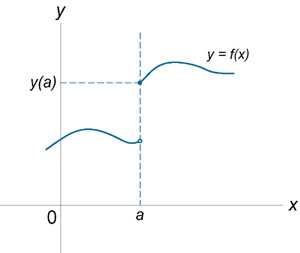
\includegraphics{fig1.jpg}
% \caption{Разрыв функции}
% \label{разрыв_функции}
% \end{figure}


% У заключения нет номера главы
\section*{Заключение}
В данной работе...\cite{DESMAN}


\bibliographystyle{ugost2008ls}
\bibliography{diploma.bib}
\end{document}
